\def\VCDate{2015/10/07}\def\VCVersion{(Current)}
\documentclass{article}
\usepackage[screen]{geometry}
\usepackage{ProofPower, graphicx, amsmath}
\begin{document}
\title{Lab 2}
\author{Ai Nguyen}
\maketitle
\clearpage
\section{GCD in Math}
\par This lab explores how we can create and use functions in the three different languages focused on in this course: SML, C, and ASM. The function we will be trying to implement is GCD, or the greatest common divisor of two positive integers.
\par This should give us the largest number that is exactly divides both of them such that there is no remainder. For example, the GCD of 14 and 12 is 2 and the GCD of 14 and 11 is 1.

The GCD is given by the following specification:
\[ gcd: \mathbb{N} \times \mathbb{N} \rightarrow \mathbb{N}\]
\[ gcd(m,n) = max \{d \in \mathbb{N} \vert m \bmod d = 0 \land n \bmod d = 0\}\]
One algorithm for calculating the gcd follows Euclid's method. If, for 2 natural numbers m and n, if m $>$ n, then the gcd is defined by:
\[ euclid(m,n) = \left\{ \begin{array}{l}
                        euclid(n,m \bmod n), \text{if n $>$ 0}\\
                        m
                        \end{array} 
\right. \]
\clearpage
\section{GCD in SML}
The GCD can be implemented in SML like this:
\begin{GFT}{SML}
\+fun euclid (m, n) = if n > 0 then euclid (n, (m mod n))\\
\+		else m;\\
\+euclid(14,12);\\
\+euclid(14,11);\\
\+euclid(558,198);\\
\end{GFT}
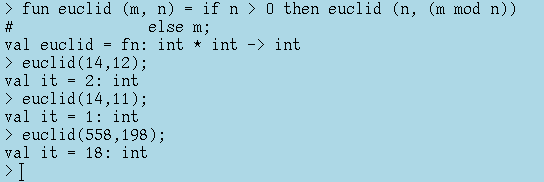
\includegraphics[scale = 0.6]{gcd_sml.png}\\
Since SML is naturally a functional and mathematics based language, it is quite easy to implement the GCD function in SML.

\clearpage
\section{GCD in C}
GCD can also be implemented in C. The following recursive function is a very simple and effective implementation of the Euclid method of getting the greatest common divisor 
\begin{GFT}{C source code written to file lab2.c}
\+\#include<stdio.h>\\
\+int euclid(int m, int n)\{\\
\+  if(n > 0) return euclid(n, m \% n);\\
\+  else return m;\\
\+\}\\
\end{GFT}

Let's try to write an equivalent function that is more like ASM. For example,
do not use function composition. Do each operation on a separate line. 
\begin{GFT}{C source code appended to file lab2.c}
\+int euclidasm(int m, int n)\{\\
\+  int r;\\
\+  if (n>0)\\
\+    r = euclid(n,m \%n);\\
\+  else \\
\+    r = m;\\
\+  return r;\\
\+\}\\
\end{GFT}
Now we can test the two functions and see if they both work.
\begin{GFT}{C++ source code appended to file lab2.c}
\+int main()\\
\+\{\\
\+  printf("\%d\Backslash{}n", euclid(14,12));\\
\+  printf("\%d\Backslash{}n", euclid(14,11));\\
\+  printf("\%d\Backslash{}n", euclid(558,198));\\
\+  printf("The euclid-asm version of the previous line: \%d\Backslash{}n", euclidasm(558,198));\\
\+\}\\
\end{GFT}
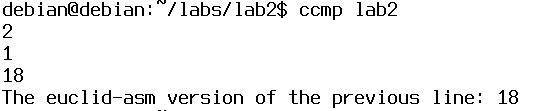
\includegraphics[scale =0.5]{gcd_c.png}
\par When we run the program, we get the same results as SML gives us, (2, 1, 18), which is a good sign. Note that the C implementation is similar to the SML implementation in which we give a clear algorithm for calculating the GCD (if, else...). 

\clearpage
\section{GCD in ASM}
\par Although these previous implementations are direct translations from math to SML to C, it is difficult to continue onto ASM because of the one-to-many relationship between C and ASM (and IA32 instruction set). For example, ASM does not have direct support for function composition. \\
So instead of doing something like this: \\
\verb|printf("%d\n", euclid(558,198));| \\
In ASM we have to do something more like this:
\begin{verbatim}
  int t = euclid(558/198);
  printf("%d\n"",t);
\end{verbatim}

However this is not possible since we can't assign a returned value into a memory location. Instead we always put it in the eax register for return values.
\begin{GFT}{asm source code written to file lab2.s}
\+.data \\
\+  fmt: .string "\%d\Backslash{}n" \\
\+.text                 \\
\+.global \_start  \\
\end{GFT}
\clearpage
The following code calculates euclid(558,198) and prints it to the screen
\begin{GFT}{asm source code appended to file lab2.s}
\+\_start:            \\
\+  push \$198        \\
\+  push \$558\\
\+  call euclid      \\
\+  add \$8, \%esp     \\
\+  push \%eax\\
\+  push \$fmt         \\
\+  call printf    \\
\+  add \$8, \%esp\\
\end{GFT}
Since we have finished printing the output of euclid, we can now end the program
\begin{GFT}{asm source code appended to file lab2.s}
\+  mov \$1, \%eax  \\
\+  mov \$0, \%ebx\\
\+  int \$0x80    \\
\end{GFT}
\clearpage
Definition of Euclid function. Problems to solve:
\begin{itemize}
\item Create stack frame for function call (use the ebp (``base pointer''), in conjunction with esp (``stack pointer''))
\item Get parameters from frame (by indirect accesing mode using offests from ebp)
\item Calculate modulus (remainder after integer division using idiv command)
\item Implement if/else statement (using cmp and jump instructions)
\item Call euclid recursively
\item Assign a return value (use mov instruction to move into eax)
\end{itemize}
\begin{GFT}{asm source code appended to file lab2.s}
\+euclid:\\
\+  push \%ebp          \\
\+  mov \%esp,\%ebp  \\
\+   mov 8(\%ebp),\%eax  \\
\+   mov \$0, \%edx      \\
\+   mov 12(\%ebp),\%ebx \\
\+  cmp \$0,\%ebx\\
\end{GFT}
\clearpage
After setting up the registers for integer division, we can check if we need to call euclid again if n is not greater than 0.
\begin{GFT}{asm source code appended to file lab2.s}
\+ jng \_else\\
\+\\
\+   idiv \%ebx \\
\+   push \%edx\\
\+   push \%ebx\\
\+   call euclid\\
\+   add \$8, \%esp\\
\+\\
\+ jmp endif\\
\+\_else: \\
\end{GFT}
In each call of euclid, we set m into eax. So if we run the function and we find that immediately n = 0, we can simply return m by calling ret. 
\begin{GFT}{asm source code appended to file lab2.s}
\+endif:\\
\+  mov \%ebp,\%esp  \#move stack pointer back onto the main stack\\
\+  pop \%ebp     \# remove the old \%ebp (which is on top)\\
\+  ret\\
\+\\
\end{GFT}
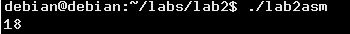
\includegraphics{lab2asm.png}
\section{Stack Frame}
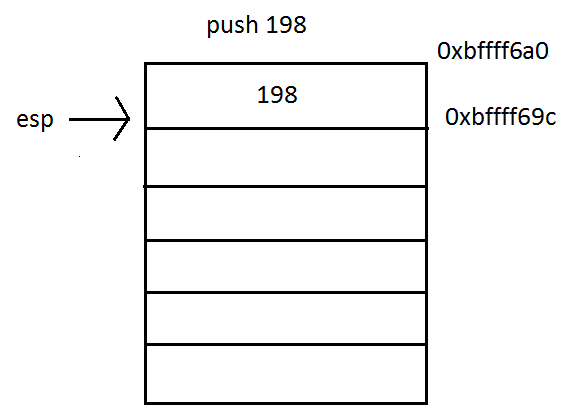
\includegraphics[scale=0.5]{stack1.png}
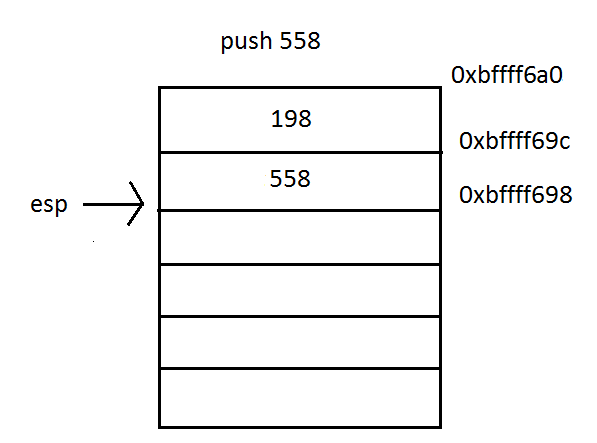
\includegraphics[scale=0.5]{stack2.png}\\
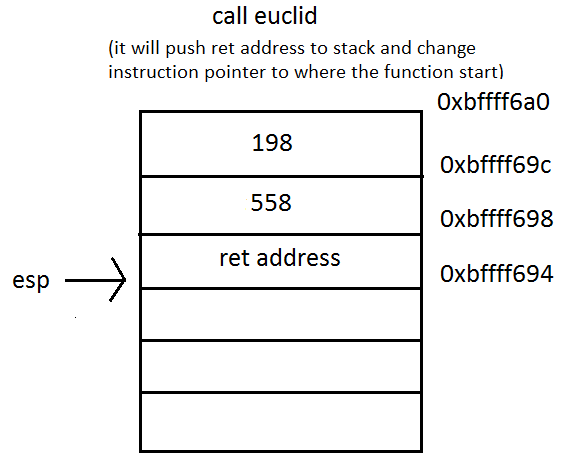
\includegraphics[scale=0.5]{stack3.png}
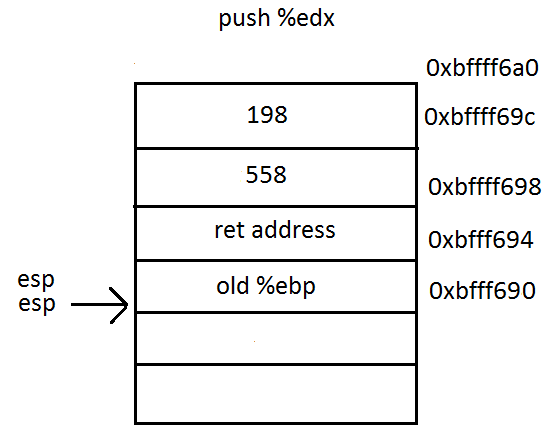
\includegraphics[scale=0.5]{stack4.png}\\
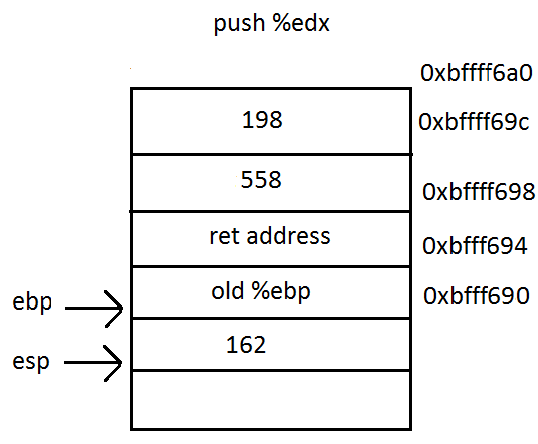
\includegraphics[scale=0.5]{stack5.png} 
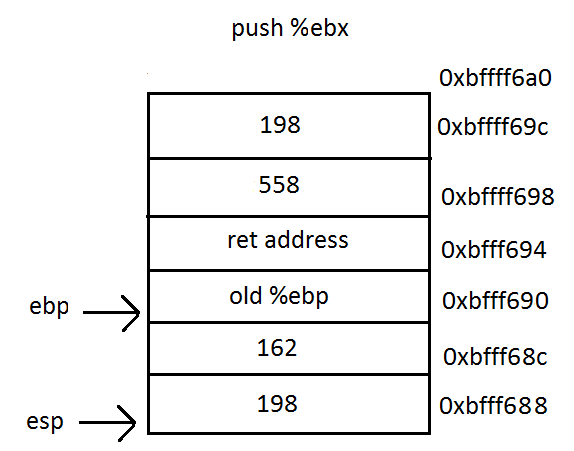
\includegraphics[scale=0.5]{stack6.png}\\
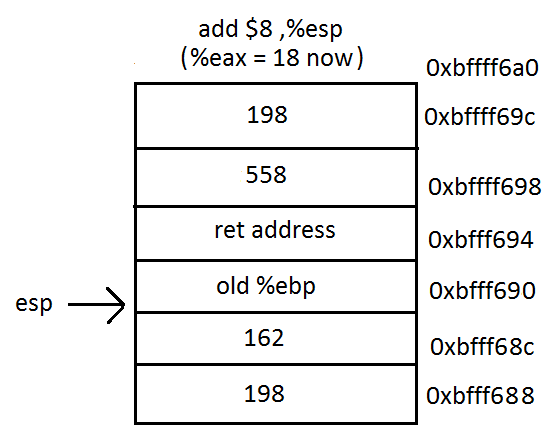
\includegraphics[scale=0.5]{stack7.png}  
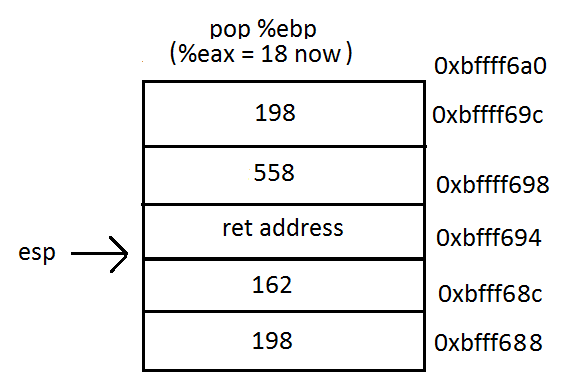
\includegraphics[scale=0.5]{stack8.png}\\
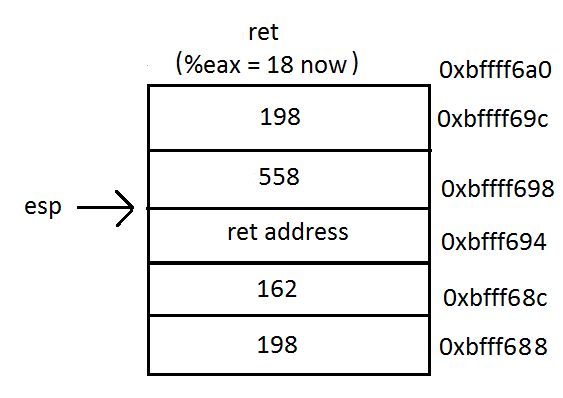
\includegraphics[scale=0.5]{stack9.png}  
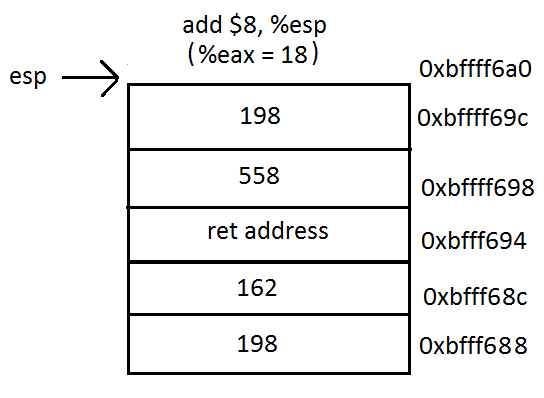
\includegraphics[scale=0.5]{stack10.png}\\
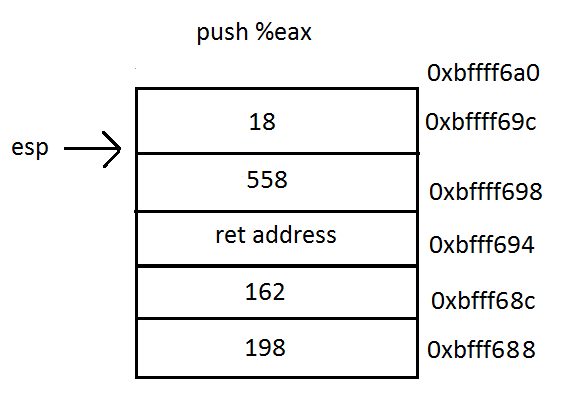
\includegraphics[scale=0.5]{stack11.png} 
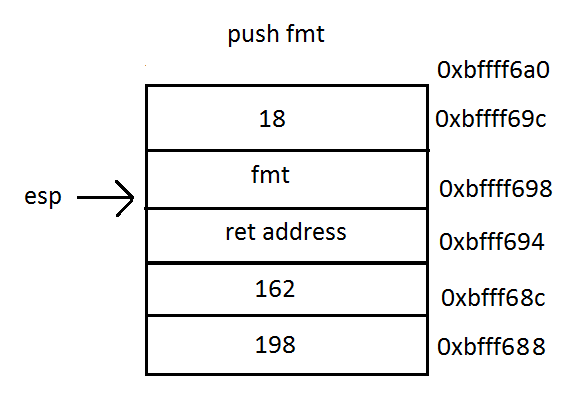
\includegraphics[scale=0.5]{stack12.png}\\
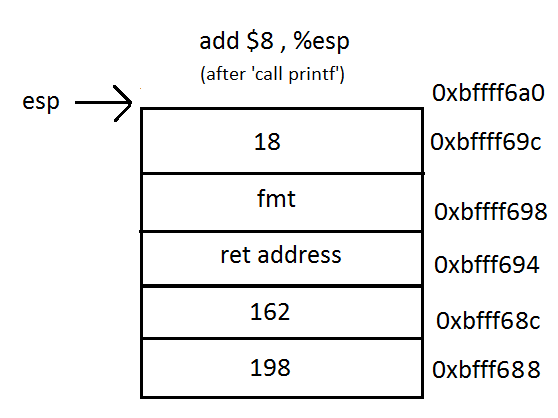
\includegraphics[scale=0.5]{stack13.png} 
\end{document}
